%!TEX root = main.tex
%
\begin{table}[h]
	\resizebox{1.01\columnwidth}{!}{%
		\centering\begin{tabular}{clcclllc}\toprule
			&        &                         &                         & Qualification   & Protected & Protected \\
			& Dataset & \multicolumn{1}{c}{$n$} & \multicolumn{1}{c}{$k$} & criterion & groups     & \% \\
			\midrule
			D1 & COMPAS \cite{angwin_2016_machine}& 6173 & 1500 & ad-hoc score & PoC & 65.9\% \\
			\midrule
			D2 & COMPAS \cite{angwin_2016_machine}& 6173 & 500 & ad-hoc score & 25yr. < x < 45yr. & 57.2\% \\
			& & & & & < 25yr. & 21.8\% \\
			\midrule
			D3 & COMPAS \cite{angwin_2016_machine}& 6173 & 200 & ad-hoc score & PoC female, < 25yr. & 2.8\%\\
			& & & & & white female, < 25yr. & 1.2\% \\
			& & & & & PoC male, < 25yr. & 13.4\% \\
			\midrule
			D4 & German credit \cite{lichman_2013_uci} & 1000 & 50 & credit rating & female, non-prot. age & 21.7\% \\
			& & & & & male, oldest 10\% & 6.3\% \\
			& & & & & male, youngest 10\% & 4.4\%  \\
			& & & & & female, oldest 10\% & 3.2\% \\
			& & & & & female, youngest 10\% & 6.1\% \\
			\midrule
			D5 & LSAT \cite{wightman1998lsac}  & 21K & 200  & LSAT score  & White, female & 35.3\%  \\
			& & & & & PoC, female & 8.4\% \\
			& & & & & PoC, male & 7.6\% \\
			\bottomrule
		\end{tabular}
	}
	\caption{Datasets and experimental settings. The ad-hoc score for COMPAS was calculated by a weighted summation of recidivism risk, number of prior arrests and violent recidivism risk.	\label{tbl:datasets}}
	\vspace{-3mm}
\end{table}
%
\section{Experiments}\label{sec:experiments}
%\todo{Are we still doing this experiment to verify algorithm correctness?}
%In the first part of our experiments we create synthetic datasets to demonstrate the correctness of the adjustment done by Algorithm \algoCorrect (\S\ref{subsubsec:JuliaExperimentalVerification}).
%
In this section, we consider several reference datasets for evaluating the multinomial \algoFAIR algorithm (datasets in \S\ref{sec:experiments-datasets}, metrics and comparison with baselines in \S\ref{sec:experiments-baselines}, and results in \S\ref{sec:experiments-results}).

\begin{figure}[t]
	\vspace{-8mm}
	\centering
	\subfloat%
	[Score distribution of male and female candidates in the COMPAS dataset.
	\label{fig:dataset:compas:sex}]
	{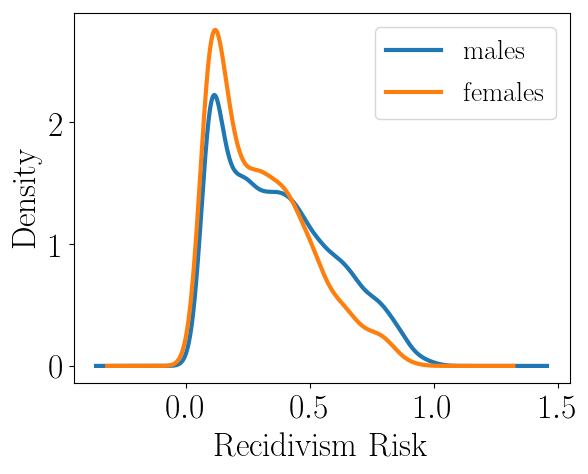
\includegraphics[width=.48\textwidth]{pics/compas_sex_kde.png}}\hfill
	\subfloat
	[Score distribution of white and non-white candidates in the COMPAS dataset. Experiment D1.
	\label{fig:dataset:compas:race}]
	{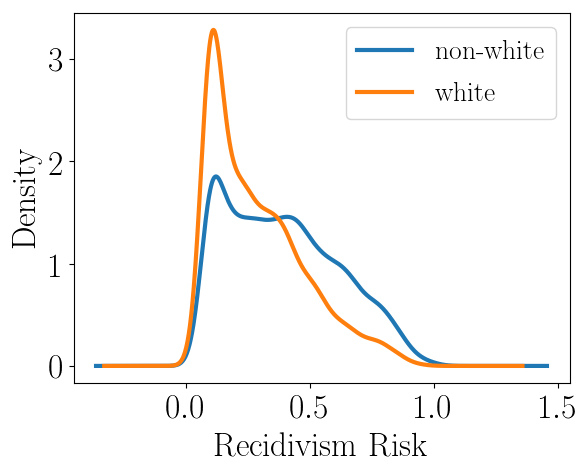
\includegraphics[width=.48\textwidth]{pics/compas_race_kde.png}}\hfill
	\subfloat
	[Score distribution by age in the COMPAS dataset \inote{older THAN 45 or $>45$, younger THAN 25 or $<25$}. We see that age is a strong predictor of recidivism risk which suggests that the COMPAS questionnaire injects a bias against younger people into the data. Experiment D2.
	\label{fig:dataset:compas:age}]
	{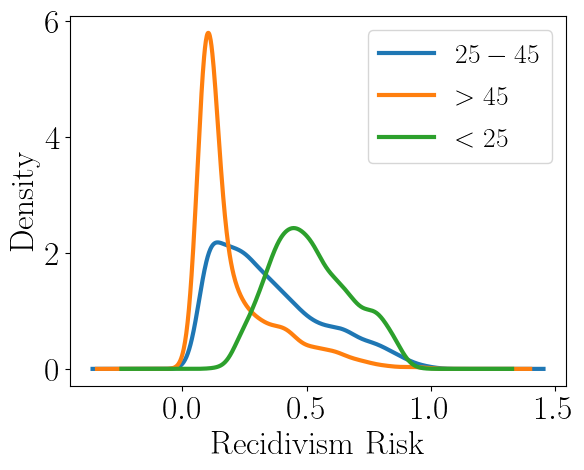
\includegraphics[width=.48\textwidth]{pics/compas_age_kde.png}}\hfill
	\subfloat
	[Score distribution protected and non-protected candidates in the COMPAS dataset. Protected groups are young non-white males, young non-white females and young white females, which are the three groups with lowest average exposure in the colorblind ranking. Experiment D3.
	\label{fig:dataset:compas:worstThree}]
	{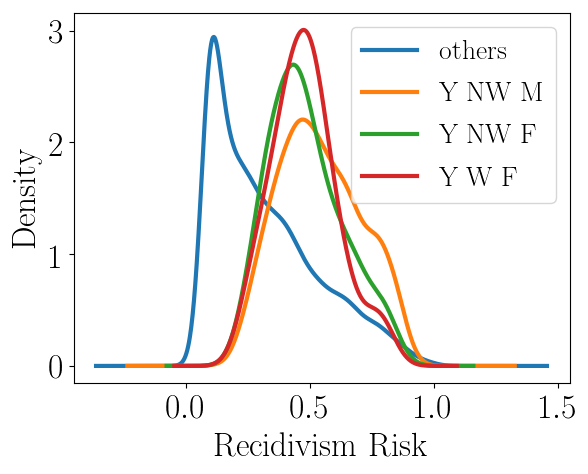
\includegraphics[width=.48\textwidth]{pics/compas_worstThreeGroups_kde.png}}\hfill
	\vspace{-3mm}
	\caption{Distribution of COMPAS scores in different experimental settings. The first three figures show distributions separately by each of the three protected categories. The fourth figure shows the distribution for dataset D3}
	\label{fig:dataset:compas}
	\vspace{-3mm}
\end{figure}

\subsection{Datasets}\label{sec:experiments-datasets}

\note[ChaTo]{I'm uncomfortable with using ``quality'' -- throughout the paper, I would refer to this as simply ``score''.}

Table~\ref{tbl:datasets} summarizes the datasets used in our experiments.
%
Each dataset contains a set of people with demographic attributes, plus a score attribute.
%
Note that dataset D1 is the same experimental setup as in our previous paper~\cite{zehlike2017fair}, but instead of using the original algorithm \algoFAIR, we run the binomial experiment with the multinomial extension proposed in Section~\ref{sec:problem}.
%
For each dataset, we consider a value of $k$ that is a round number ({\em e.g.}, 50, or 200) with $k<n$.
%
For the purposes of these experiments, we considered several scenarios of protected groups.
%
We remark that the choice of protected group is not arbitrary: it is determined completely by law or voluntary commitments; for the purpose of experimentation we test different scenarios, but in a real application there is no ambiguity about which is the protected (historically and currently disadvantaged) group.
%
Similarly, the minimum proportion can always be provided by regulation or voluntary commitments; in the absence of this minimum proportion one can use the fraction of people who are members of that group within the entire population.
%
An experiment consists of generating a \inote{re-?}ranking using multinomial \algoFAIR and then comparing it with baseline rankings according to the metrics introduced in the next section.
%
We use the three publicly-available datasets: COMPAS~\cite{angwin_2016_machine}, German Credit~\cite{lichman_2013_uci}) and LSAC~\cite{wightman1998lsac}.

\spara{COMPAS} (Correctional Offender Management Profiling for Alternative Sanctions) is an assessment tool for predicting recidivism based on 137 items/questions. It is used in several jurisdictions in the US, and has been accused of racial discrimination by having a larger false positive rate for African Americans~\cite{angwin_2016_machine}.
%
In our experiment, we test a scenario in which we want to create a fair ranking of the top-$k$ people who are least likely to recidivate, who could be, for instance, considered for an alternative program to prison.
%
We calculated a candidate's overall score as a weighted summation of the columns ``recidivism, violent recidivism'' and ``prior arrests'' from the original dataset.
%
To break ties we added normally distributed random noise with $\mu=0, \sigma=0.00001$ to the score of each candidate.
%
Our protected groups are formed by different combination of the attributes ``race, age'' and ``sex'', where race is either ``white'' or ``non-white'', age is either ``younger than 25'', ``between 25 and 45'' or ``older than 45'', and sex is either ``male'' or ``female''.
%
We observe in Figure~\ref{fig:dataset:compas} that non-white people (\ref{fig:dataset:compas:race}), as well as males (\ref{fig:dataset:compas:sex}) are given a larger recidivism score than other groups.
%
However we see in Figure~\ref{fig:dataset:compas:age} that the protected attribute ``age'' has the strongest impact on recidivism risk.
%
Apparently COMPAS tends to give larger risk scores to younger people.
%
We therefore consider white, female and older than 45 as the \emph{non-protected} categories for our experiments.


In dataset D1 we consider people of color as the protected group and conduct experiments with two different minimum proportion vectors.
%
The first one sets the $p$-values to match the protected group proportion in the dataset $p_{\text{stat}}=[0.66]$ which relates to group fairness as statistical parity; the second one sets all minimum proportions to the same value $p_{\text{eq}}=[0.5]$.


In dataset D2 we consider people aged 25--45 and younger than 25 as protected and the vectors $p_G$ are $p_{\text{stat}}=[0.573,0.218]$ and $p_{\text{eq}}=[0.333, 0.333]$.


In dataset D3 we divided the candidates into 12 different groups that we constructed from the Cartesian product of all three protected categories ``age,'' ``race,'' and ``sex''.
%
Then we calculated the average group exposure for each group and considered as protected the three groups that were placed lowest in the colorblind ranking.
%
These are young non-white females, young white females and young non-white males.
%
Interestingly, despite the fact that females have higher scores on average, two of the three groups with lowest exposure values are female (Figure~\ref{fig:dataset:compas:worstThree}).
%
We set the vectors $p_G$ to $p_{\text{stat}}=[0.028,0.012,0.134]$ and $p_{\text{eq}}=[0.25,0.25,0.25]$.


\spara{German Credit} is the Statlog German Credit Data collected by Hans Hofmann~\cite{lichman_2013_uci}.
%
It is based on credit ratings generated by \emph{Schufa,} a German private credit agency based on a set of variables for each applicant, including age, gender, marital status, among others. The Schufa score is an essential determinant for every resident in Germany when it comes to evaluating credit rating before getting a phone contract, a long-term apartment rental or almost any loan.
%
We use the credit-worthiness as qualification, calculated as a weighted summation of the features account status, credit duration, credit amount and employment length.
%
As protected attributes we use the sex and age of a candidate: females and whether or not they belong to the group of the 100 youngest or oldest persons respectively form the protected groups, because these tend to be given lower scores.
%
We set the vectors $p_G$ to $p_{\text{stat}}=[0.217,0.063,0.044,0.032,0.061]$ and $p_{\text{eq}}=[0.166,0.166,0.166,0.166,0.166]$.


\spara{LSAT} is a dataset collected by~\citet{wightman1998lsac} to study whether the admission metrics to law schools in the US have a disparate impact on students of color.
%
The qualification attribute consists of scores in the US Law School Admission Test (LSAT).
%
The protected features are a person's sex and whether or not they belong to the group of people of color (PoC).
%
Women and PoC score on average lower than men and Whites in this test, which is why we regard white men as non-protected and the other groups as protected.
%
We set the vectors $p_G$ to $p_{\text{stat}}=[0.353,0.084,0.076]$ and $p_{\text{eq}}=[0.25,0.25,0.25]$.


\subsection{Baselines and Metrics}\label{sec:experiments-baselines}

For each dataset, we generate various top-$k$ rankings with varying targets of minimum proportion of protected candidates $p$ using \algoFAIR, plus two baseline rankings:

\spara{Baseline 1: Color-blind ranking.} The ranking $\textit{cb}|_k$ that only considers the scores/qualifications of the candidates, without considering group fairness, as described in Section~\ref{concept:color-blind-ranking}.

\spara{Baseline 2: \citet{zehlike2020matching}.} The Continuous Fairness Algorithm (CFA$\theta$) is a post-processing ranking method that aligns the score distributions of the protected candidates with the Wasserstein-barycenter of all group distributions.
%
To achieve this the algorithm finds a new distribution of scores for each group, the "fair representation", by interpolating between the barycenter and the group distribution, subject to a given fairness parameter $\theta$.
%
This fair representation corresponds to the idea to rank groups separately and then subsequently pick the best candidates from each group to create the result ranking.
%
Note that setting $\theta=1$ to its maximum corresponds to setting the minimum proportions in $p_G$ to the dataset proportions of each group.
%
This means that with CFA$\theta$ we can not achieve an exposure gain that would require minimum proportions beyond statistical parity.
%
Hence this method is comparable to our method only if all values in $p_G$ are less or equal to statistical parity.
%
In our experiments we therefore only compare \algoFAIR with $p_{\text{stat}}$ to CFA$\theta$ with $\theta=1$, as higher $p$-values are not comparable.


\spara{Utility (Performance Measure). } We report the loss in ranked utility after score normalization, in which all $q_i$ are normalized to be within $[0, 1]$.
%
We also report the maximum rank drop, {\em i.e.}, the number of positions lost by the candidate that realizes the maximum ordering utility loss.


\spara{NDCG (Performance Measure). }
%
We report a normalized weighted summation (Normalized Discounted Cummulative Gaing - NDCG) of the scores of the elements in the ranking, $\sum_{i=1}^{k} w_i q_{(\tau_i)}$, in which the weights are chosen to have a logarithmic discount in the position:  $w_i = \frac{1}{\log_2 (i+1)}$. This is a standard measure to evaluate search rankings~\cite{jarvelin2002cumulated}.
%%
This is normalized so that the maximum value is $1.0$.


\spara{Exposure (Fairness Measure). } We use a measure of average group exposure, which we define as the average position bias that a group is exposed to.
%
In rankings, their exposure to the user is critical for ranked candidates to benefit from the system and if a group of candidates is systematically ranked low, it can be considered as biased~\cite{friedman1996bias}.
%
We model position bias $v$ by means of a logarithmic progression of the form $v(k) = \frac{1}{\log_2(i+1)}$.
%
Thus the first position has a bias $v(1)=1$, which then decreases logarithmically.
%
Higher position bias translates into more exposure and hence more visibility.
%
We show that large increases in average group exposure can be achieved with relatively small losses in ordering utility and NDCG.


\subsection{Results}\label{sec:experiments-results}
%
\begin{table}[b!]
	\resizebox{1.02\columnwidth}{!}{%
		\centering\begin{tabular}{lccccc}\toprule
				   & Exposure &   total    & Ordering     & Rank & Selection \\
			Method & gain per group & NDCG loss  & utility loss & drop & utility loss \\

			\midrule
			\multicolumn{6}{c}{D1 -- COMPAS, k=1500, race (1 prot.)} \\
			\midrule
			\algoFAIR $p_{\text{eq}}$ & $[-0.27, 0.27]$ & $1.915\cdot10^{-7}$ & $[0.0066, 0]$ & $[15, 0]$ & $[0, 0]$ \\
			\algoFAIR $p_{\text{stat}}$ & $[-19.16, 19.16]$ & 0.0039 & $[0.0687, 0]$ & $[387, 0]$ & $[0.0621,0]$ \\
			\citeauthor{zehlike2020matching} & $[-28.6, 28.6]$  & 0.0055 & $[0.0738, 0]$ & $[620, 288]$ & $[0.0702, 0]$ \\

			\midrule
			\multicolumn{6}{c}{D2 -- COMPAS, k=500, age (2 prot.)} \\
			\midrule
			\algoFAIR $p_{\text{eq}}$ & $[-13.77, -7.10, \textcolor{red}{20.87}]$ & 0.0580 & $[0.23, 0,23, 0.00]$ & $[182, 127, 0]$ & $[0.23, 0.23, 0.00]$ \\
			\algoFAIR $p_{\text{stat}}$ & $[-20.86, 6.75, \textcolor{red}{14.11}]$ & 0.0354 & $[0.21, 0.21, 0.00]$ & $[266, 3, 0]$ & $[0.21, 0.21, 0.00]$ \\
			\citeauthor{zehlike2020matching} & $[-38.48, 18.11, \textcolor{red}{20.49}]$ & 0.0521 & $[0.19, 0.18 ,0.00]$ & $[159, 280, 0]$ & $[0.19, 0.17, 0,00]$ \\ %\cline{2-7}

			\midrule
			\multicolumn{6}{c}{D3 -- COMPAS, k=200, three worst off (3 prot.)} \\
			\midrule
			\algoFAIR  $p_{\text{eq}}$ & $[-21.87, \textcolor{red}{7.29}, \textcolor{red}{7.30}, \textcolor{red}{7.27}]$ & 0.1526 & $[0.42, 0.14, 0.00, 0.22]$ & $[134, 0, 0, 0]$ & $[0.42, 0.13, 0.00, 0.22]$ \\
			\algoFAIR  $p_{\text{stat}}$ & $[-3.62, \textcolor{red}{0.60}, \textcolor{red}{0.29}, \textcolor{red}{2.73}]$ & 0.0155 & $[0.17, 0.03,0.00, 0.02]$ & $[24, 0,0,0]$ & $[0.17, 0.00,0.00, 0.02] $  \\
			\citeauthor{zehlike2020matching} &  $[-11.83, \pm 0, \pm 0, \textcolor{red}{11.83}]$ & 0.0562 & $[0.19, \pm 0, \pm 0, 0.00] $ & $[178, \pm 0, \pm 0, 0]$ & $[0.19, \pm 0, \pm 0, 0.00]$   \\

			\midrule
			\multicolumn{6}{c}{D4 -- German credit, k=50, sex \& age (5 prot.)} \\
			\midrule
			\algoFAIR $p_{\text{eq}}$ &  $[-4.46, 0.08, 0.50, $ & 0.1698 & $[3.51, 2.70, 3.42, $ & $[28, 4, 7, 1, 0, 0]$ & $[3.05, 1.82, 1.34, $\\
			& $1.49, 1.26, 1.12]$ & &  $ 0.55, 1.18, 1.76]$& & $0.00, 0.18, 0.33]$  \\
			\algoFAIR $p_{\text{stat}}$ &  $[-0.83, 0.01, 0.23, $& 0.0185 & $[1.84, 1.56, 0.45, $ & $[5, 3, 1, 0, 0, 5]$ & $[1.89, 1.56, 1.23,$  \\
			& $0.38, 0.20, 0.01]$  & & $0.00, 0.33, 1.28]$ & & $ 0.00, 1.18, 1.54]$\\
			\citeauthor{zehlike2020matching} &  $[1.15, 0.22, -0.91, $ & 0.0471 & $[0.50, 1.41, 2.06,$ & $[2, 2, 31, 22, 0, 0]$ & $[0.34, 0.00, 1.93, $ \\
			& $-0.71, 0.00, 0.25]$ &  & $ 1.75, 0.27, 0.00]$ & & $2.20, 0.00, 0.00]$\\

			\midrule
			\multicolumn{6}{c}{D5 -- LSAT, k=200, sex \& race (3 prot.)} \\
			\midrule
			\algoFAIR $p_{\text{eq}}$ & $[-15.76, -1.48, 8.41, 8.82]$ & 0.0157 & $[4,4,1,0]$ & $[145, 28, 0, 0]$ & $[4, 4, 1, 0`]$  \\
			\algoFAIR $p_{\text{stat}}$ & $[-11.12, 3.87, 2.80, 4,44]$ & 0.0026 & $[2, 2, 1, 0]$ & $[100, 15, 0, 0]$ & $[2, 2, 1, 0]$  \\
			\citeauthor{zehlike2020matching} &  $[-14.63, 4.29, 3.88, 6.46]$ & 0.0049 & $[2, 1, 1, 0]$ & $[149, 26, 0, 0]$ & $[2, 1, 0, 0]$  \\

			\bottomrule
		\end{tabular}
	}
	\caption{Experimental results, expressed in terms of changes of exposure and utility with respect to colorblind results.
		%
		%Colorblind results are not shown because they are always zero.
		%
		All measures are presented per group except for the loss of NDCG which is calculated for the entire ranking.
		%
		Groups are in the same order as in Table~\ref{tbl:datasets}, and the first value is always for the non-protected group.
		%
		With $p_{\text{stat}}$ we denote a vector $p_G$ that contains the share of a group as its $p$-value, hence the produced ranking should obtain statistical parity.
		%
		With $p_{\text{equal}}$ we denote a vector $p_G$ that contains the same value for all $p$.
		%
		For exposure gain we report numbers in red, if a group was not among the top-$k$ in the colorblind ranking, but is now.
		%
		These numbers constitute the absolute exposure value a group receives after re-ranking.
		%
		We write $\pm 0$, if the group appears neither in the colorblind, nor in the fairly re-ranked top-$k$.
		%
		We observe that \algoFAIR $p_{\text{stat}}$ and the baseline CFA$\theta$ have comparable results for experiments D1 and D5.
		%
		However, we also see that CFA$\theta$ seems to not handle ties well in experiments D2 and D3 (see textual explanation for details).
		%
		For experiment D4 we see an interesting property of \algoFAIR: the youngest and oldest males experience a high rank drop (31 and 22) with CFA$\theta$ compared to \algoFAIR $p_{\text{stat}}$, even though they belong to the protected groups.
		%
		This is because they receive exposure values higher than average in the $cb|_k$, i.e. these two groups have the best scores.
		%
		CFA$\theta$ moves \emph{all} score distributions towards the barycenter and thus, removes the advantage that the protected groups have in this data set.
		%
		\algoFAIR, in contrast, ranks candidates based on their scores, as soon as the ranked group fairness conditions are met for each group.
		%
		As such, a protected group can only lose exposure for another protected group, but never for the non-protected one.
	}
	\vspace{-3mm}
	\label{tbl:results}
\end{table}
%
Table~\ref{tbl:results} summarizes the results.
\note[ChaTo]{I would use ``CFA$\theta$'' instead of Zehlike et al. in the table.

Exposure gain per group: I would split into two columns. First, ``Exposure change (non-protected group)'', ``Exposure change (protected groups)''

Red color seems to indicate something is wrong while the opposite is true,  perhaps you can underline those values or add an asterisk to them (something you can see in black and white).

The discussion about the table is split between the caption of the table and the main text. I think the caption of the table should be just to explain what each column is. The commentary and observations should appear in the main text.

As an idea, perhaps the table could be separated in two parts: first a table only with method, exposure change, NDCG change; then another table with method, ordering utility, rank drop, selection utility. The discussion following these two tables could be more easy to follow, perhaps.

}
%
We report on the result for \algoFAIR using $p_G$ in two different settings, namely as a statistical parity vector i.e. the $p$-values for each group correspond to their respective proportions in the dataset ($p_{\text{stat}}$), and as a vector with all $p$-values being equal ($p_{\text{eq}}$).
%
The actual values for $p_G$ are given in the dataset descriptions in Section~\ref{sec:experiments-datasets}.
%
Also remember that results of CFA$\theta$ are only comparable to a \algoFAIR $p_{\text{stat}}$ setting.
%
With the $p_{\text{eq}}$ setting, we illustrate the flexibility of our approach.

First, we observe that, for \algoFAIR $p_{\text{stat}}$ and CFA$\theta$, in general changes in NDCG with respect to the color-blind ranking are minor.
%
This can be explained as the utility is dominated by the top positions, which usually do not change dramatically.

Second we see that in experiments D1 and D5 \algoFAIR with $p_{\text{stat}}$ and the baseline CFA$\theta$ seem to perform more or less equally well at first glance.
%
While the former yields better numbers in terms of utility, with the latter the protected groups gain higher exposure.

Nonetheless, we found a very important drawback in the results of CFA$\theta$ in experiment D2: \citet{zehlike2020matching} does not guarantee in-group monotonicity, which we observed in our experiments.
%
Consider, for example, experiment D2, where we observe a maximum rank drop for the non-protected group of 159 for CFA$\theta$, which at first glance is less than \algoFAIR with $p_{\text{stat}}$ (266).
%
However, we found the following problems when closely investigating the result: the candidate that experienced the drop in 159 ranks was the \emph{only non-protected} candidate left in the top-500 after applying CFA$\theta$, and their original ranking position was 341 (now 500).
%
It means that the originally best candidate from the non-protected group (rank 3 in $cb|_k$) was ranked out of the top-500 by CFA$\theta$, hence the in-group ordering is not preserved.
%
We suspect that this is because the method can not handle ties well.
%
If lots of candidates have similar original scores, the fair representation scores may have large ties in which candidates are ordered randomly and not w.r.t. their original ordering.
%
In such a setting, \algoFAIR has an important advantage: it guarantees in-group monotonicity, because candidates are separated into group rankings which are sorted by decreasing qualifications.
%
No matter which group has to be picked at the current position, the respective candidate will always be the best available from that group.
%
This means while very similar scores appear to be problematic for CFA$\theta$, they are the best-scenario for \algoFAIR, because ranked-group fairness can be ensured without losing any relevance at all (NDCG stays unaffected).
%
In their work this problem is not yet described as a weakness of CFA$\theta$ by~\citet{zehlike2020matching}.

Third we observe a formerly known weakness of CFA$\theta$ manifesting in experiment D3: it can not handle data sets with very small groups or groups that show low variance.
%
For D3, note first that none of the protected candidates is part of the top-200 positions in the colorblind ranking.
%
As two of the protected groups are very small, they are not ranked into the top-200 fair ranking by CFA$\theta$, but only the largest protected group (young, male PoC) is ranked among the top-200.
%
In contrast, \algoFAIR $p_{\text{stat}}$ can handle very small groups, and gives them sufficient exposure that is in line with the minimum proportions $p_G$.
%
The same is true for experiment D4: while CFA$\theta$ can not handle the smaller groups well.
%
It increases the exposure of the non-protected group while decreasing it for the oldest males and youngest females.

For experiment D4 we observe an interesting advantage of \algoFAIR: the youngest and oldest males experience a high rank drop (31 and 22) with CFA$\theta$ compared to \algoFAIR $p_{\text{stat}}$, even though they belong to the protected groups.
%
This is because they receive exposure values higher than average in the $cb|_k$, i.e. these two groups have the best scores.
%
CFA$\theta$ moves \emph{all} score distributions towards the barycenter and thus, removes the advantage that the protected groups have in this data set.
%
\algoFAIR, in contrast, ranks candidates based on their scores, as soon as the ranked group fairness conditions are met for each group.
%
As such, a protected group can only lose exposure for another protected group, but never for the non-protected one.

Importantly, \algoFAIR allows to create rankings for user-defined values of $p$ and in particular for values beyond statistical parity, something that cannot be done directly with the baseline (\citet{zehlike2020matching} allows at maximum statistical parity in the result ranking when setting $\theta=1$, i.e. to the maximum value).

\note[ChaTo]{This part perhaps requires a subsection header or a preamble indicating why you want to introduce this new figure.

Again, perhaps in the caption of Figure~\ref{fig:results-moving-p} given that the caption is long, I would move the discussion/commentary on the results to the main text, and leave in the caption just the indication of what the number mean.}
Figure~\ref{fig:results-moving-p} shows results when varying $p_1$ and $p_2$ in data set D2 (COMPAS, the protected groups are people of age 25--45 ($p_1$) and people under 25 years ($p_2$).
%
This means that \algoFAIR allows a wide range of positive actions, for instance, granting reintegration programs to people with promising COMPAS ratings, with a preference towards younger offenders.
%
In this case, the Figure~\ref{fig:experiments:compasAge:ndcgloss} shows that we can double the proportion of young people in the top-$k$ ranking (e.g. from 0\% in the original up to 40\% in the fair ranking) without introducing a large drop for the other protected group loss: in the colorblind ranking they received exposure equivalent to $0.4 > p_1 > 0.5$, so setting $p_1 = p_2 = 0.4$ only causes an exposure drop of 5.8\%.
%
At the same time the NDCG loss is just 5.6\% and never exceeds 15\%, even when favoring young people with $p_2=0.8$.
\begin{figure}[t!]
\vspace{-5mm}
	\centering
	\subfloat[Exposure loss for the non-protected group. \label{fig:experiments:compasAge:expGain:groupNP}]{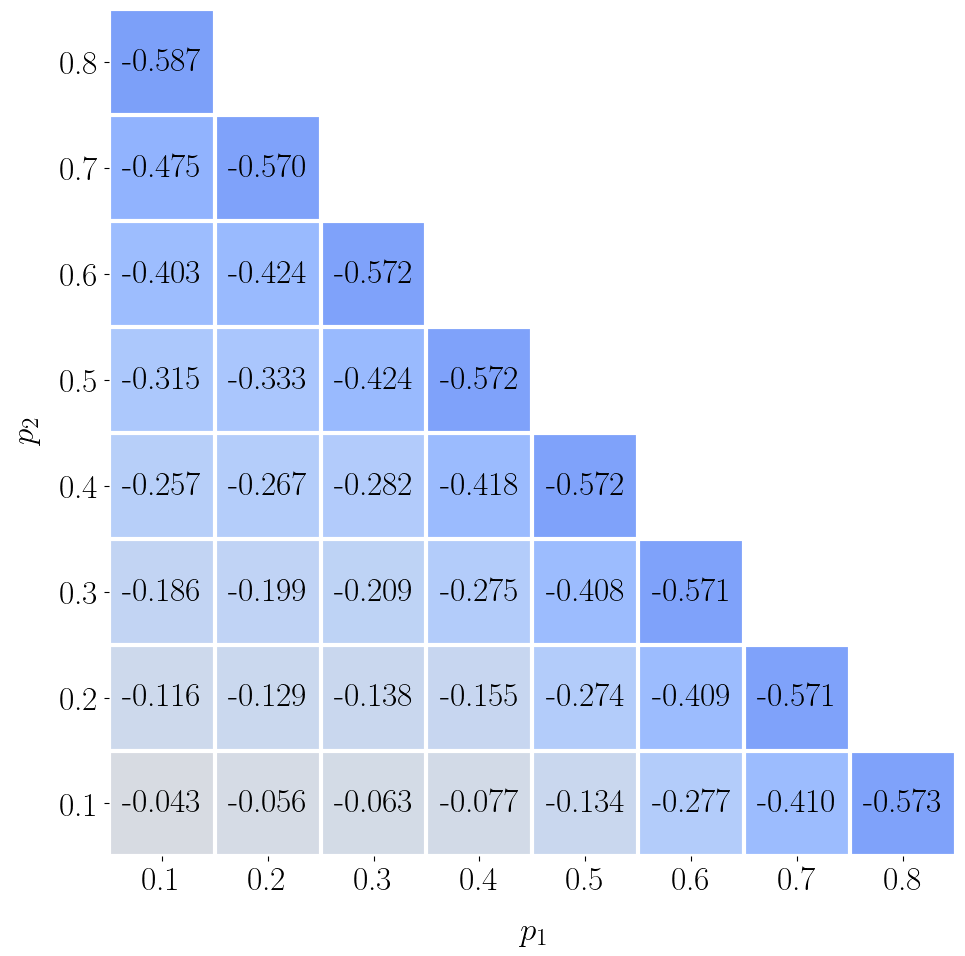
\includegraphics[width=.49\textwidth]{pics/k=200-heatmap-expGainGroupNP.png}}
	\subfloat[Exposure gain/loss for group ``age 25 -- 45''. \label{fig:experiments:compasAge:expGain:group1}]{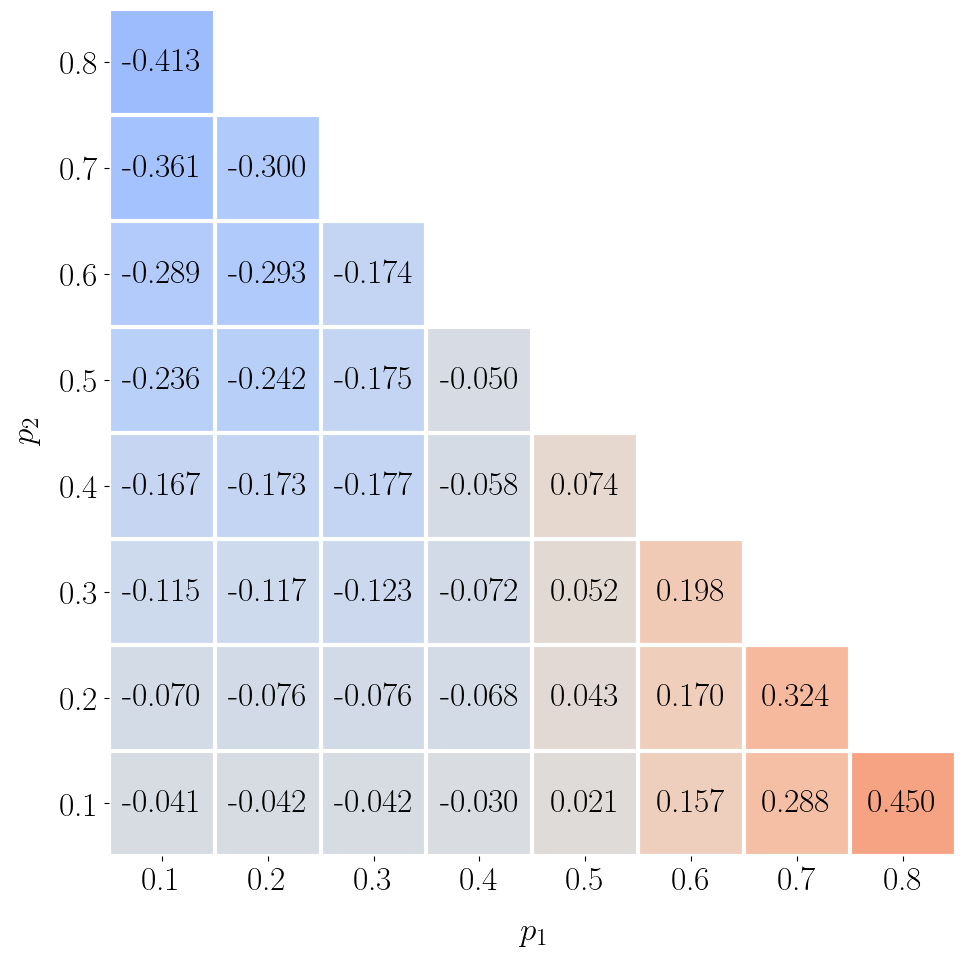
\includegraphics[width=.49\textwidth]{pics/k=200-heatmap-expGainGroup1.png}}\hfill
	\subfloat[Exposure gain for group ``age < 25''. \label{fig:experiments:compasAge:expGain:group2}]{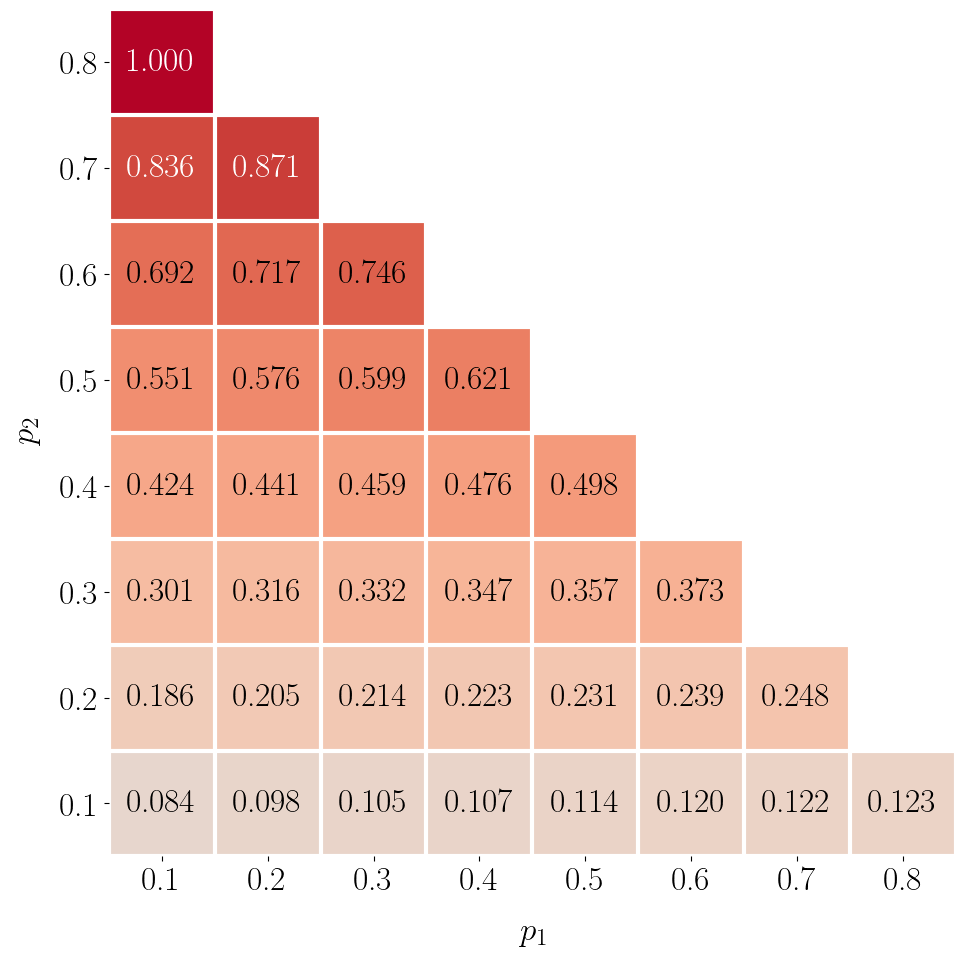
\includegraphics[width=.49\textwidth]{pics/k=200-heatmap-expGainGroup2.png}}
	\subfloat[NDCG loss. \label{fig:experiments:compasAge:ndcgloss}]{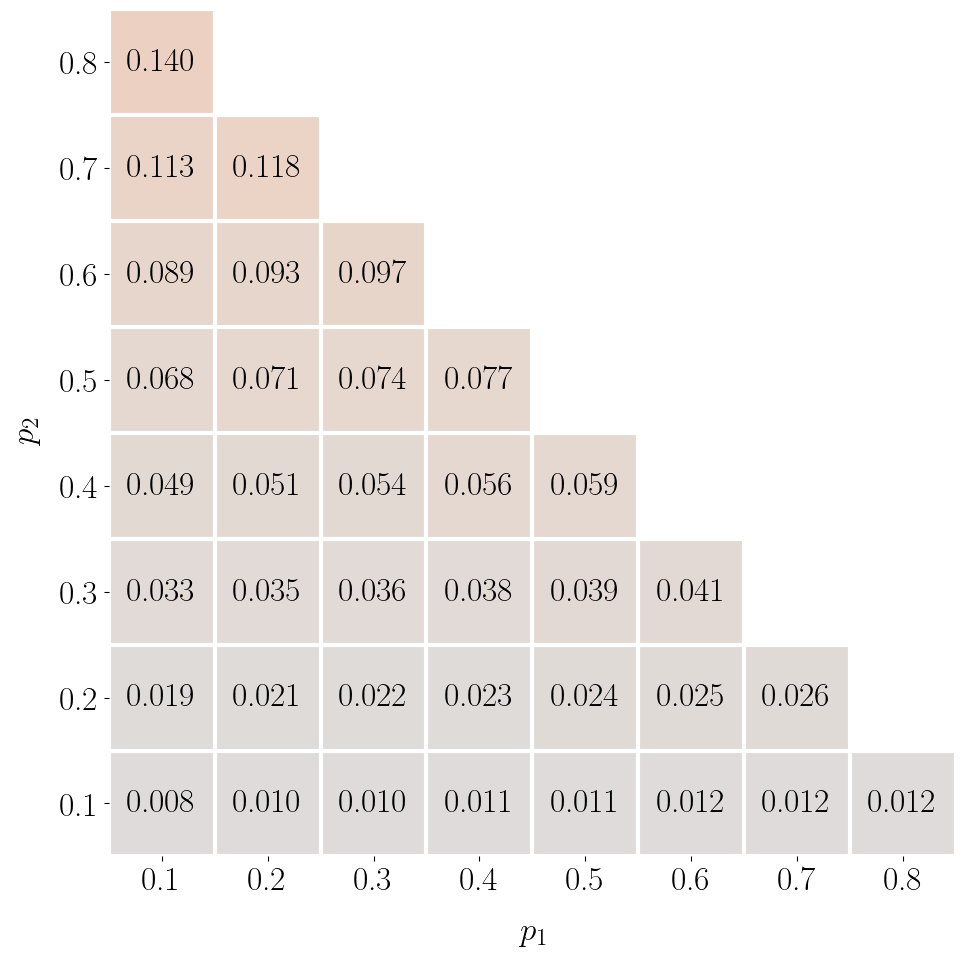
\includegraphics[width=.49\textwidth]{pics/k=200-heatmap-ndcgLoss.png}}
	\vspace{-3mm}
	\caption{Normalized exposure gain/loss and NDCG loss w.r.t. the colorblind ranking in experiment D2 (COMPAS with age as protected category) for different values of $p_1$ and $p_2$ ($k=200, \alpha=0.1$).
		%
		$p_1$ relates to group ``age 25 -- 45'', $p_2$ relates to group ``age < 25''.
		%
		Blue fields in Fig.~\ref{fig:experiments:compasAge:expGain:groupNP} -- \ref{fig:experiments:compasAge:expGain:group2} indicate that this group lost exposure w.r.t. the colorblind ranking, red fields indicate exposure gain.
		%
		In Fig.~\ref{fig:experiments:compasAge:expGain:groupNP} we see that the non-protected group loses exposure under all settings, as expected.
		%
		At the same time however NDCG loss is minor and under many settings not reaching beyond a statistical significance level of 0.05\% (Fig.~\ref{fig:experiments:compasAge:ndcgloss}).
		%
		Comparing Figures~\ref{fig:experiments:compasAge:expGain:group1} and~\ref{fig:experiments:compasAge:expGain:group2} we see that in general, if one protected group scores significantly better in the colorblind ranking (group ``25 -- 45'' in Fig.~\ref{fig:dataset:compas:age}) than another one (group ``younger 25'' in Fig.~\ref{fig:dataset:compas:age}), the first may be ranked down to make room for the second.
		%
		Figure~\ref{fig:experiments:compasAge:expGain:group1} shows that the middle-aged group in the COMPAS data set loses exposure to the young group unless $p_1$ is set high enough.
		%
		However even if $p_1$ is set low it still ensures that candidates from the middle-aged group show in the ranking, thus always losing less exposure than the non-protected group (compare Fig.~\ref{fig:experiments:compasAge:expGain:groupNP} and~\ref{fig:experiments:compasAge:expGain:group1}).
		%
		Note that this experiment is an extreme case, where no candidates from group ``age < 25'' where ranked in the top-200 in $cb|_k$, which explains why this group never loses exposure under any setting for $p_1$ and $p_2$ (see Fig.~\ref{fig:experiments:compasAge:expGain:group2}).
	}
	\vspace{-\baselineskip}
	\label{fig:results-moving-p}
\end{figure}
